\section{Activation} \label{sec:activation}
The activation function is a term that we repeatedly have used, but not really detailed. It is used to activate the outputs, which often need to take some certain properties. For instance, when doing classification, the outputs are probabilities and therefore between 0 and 1. A nonlinear activation function is often preferred to reinforce the non-linearity of the neural network. 

Traditionally, the logistic function and the tanh function have been used as activation functions, since they where believed to work in the same way as the human brain. However, in 2012 a new network was introduced known as AlexNet, taking image recognition to a new level. They used a function named Rectified Linear Units (ReLU), which is zero for negative values. Based on this, some successful activation functions have been innovated in the recent years, such as Leaky ReLU and Exponential Linear Unit (ELU). They will be examined in turn below. 

\subsection{Logistic}
The logistic activation function, also called the sigmoid function, is already mentioned several times in this report. It is widely used in classification, because it maps the outputs between 0 and 1 such that they represent probabilities for the different classes. The function reads
\begin{empheq}[box={\mybluebox[5pt]}]{align}
f(x)=\big[1+\exp(-x)\big]^{-1}.
\end{empheq}
Another important property is that the derivative has a simple form, which is just
\begin{empheq}[box={\mybluebox[5pt]}]{align}
\frac{\partial f(x)}{\partial x}=f(x)\big(1-f(x)\big)
\end{empheq}
The softmax function is like a normalized version of the logistic function. 

\subsection{ReLU}
The ReLU function is a modification of the pure linear function, where the function is pure linear for positive values and 0 else. This makes the function able to recognize the non-linearity in the model. \cite{relu} The standard ReLU function is given by 
\begin{empheq}[box={\mybluebox[5pt]}]{equation}
f(x)=
\begin{cases} 
x & \text{if} \quad x\ge 0 \\
0 & \text{if} \quad x<0.
\end{cases}
\end{empheq}
This function obviously has a clean derivative, given by the step function
\begin{empheq}[box={\mybluebox[5pt]}]{equation}
\frac{\partial f(x)}{\partial x}=
\begin{cases} 
1 & \text{if} \quad x\ge 0 \\
0 & \text{if} \quad x<0.
\end{cases}
\end{empheq}

\subsection{Leaky ReLU}
The Leaky ReLU function is again a modification of the ReLU function, but where the gradient for negative values not necessarily is zero. The function can be written as
\begin{empheq}[box={\mybluebox[5pt]}]{equation}
f(x)=
\begin{cases} 
x & \text{if} \quad x\ge 0 \\
\alpha x & \text{if} \quad x<0.
\end{cases}
\end{empheq}
This is a more general activation function, where $\alpha =1$ gives a pure linear function and $\alpha =0$ gives the standard ReLU function. Usually one wants a small derivative for negative values, setting $a$ to a small number. \cite{leaky} The derivative reads
\begin{empheq}[box={\mybluebox[5pt]}]{equation}
\frac{\partial f(x)}{\partial x}=
\begin{cases} 
1 & \text{if} \quad x\ge 0 \\
\alpha & \text{if} \quad x<0.
\end{cases}
\end{empheq}

\subsection{ELU}
Finally, we will look at the ELU function, which is another modification of the standard ReLU function. For the Leaky ReLU function, the zero gradient problem was avoided by adding a linear function with a small inclination. The idea behind ELU is similar, but the function added is an exponential function instead of a linear one. \cite{elu} The function can be written as
\begin{empheq}[box={\mybluebox[5pt]}]{equation}
f(x)=
\begin{cases} 
x & \text{if} \quad x\ge 0 \\
\alpha\big(\exp(x)-1\big) & \text{if} \quad x<0
\end{cases}
\end{empheq}
and also this has a simple derivative,
\begin{empheq}[box={\mybluebox[5pt]}]{equation}
\frac{\partial f(x)}{\partial x}=
\begin{cases} 
1 & \text{if} \quad x\ge 0 \\
f(x) + \alpha & \text{if} \quad x<0.
\end{cases}
\end{empheq}

\subsection{Illustration}
In figure (\ref{fig:activation_functions}), standard RELU, Leaky RELU and ELU are plotted along with the logistic function.

\begin{figure} [H]
	\centering
	\subfloat[Logistic]{{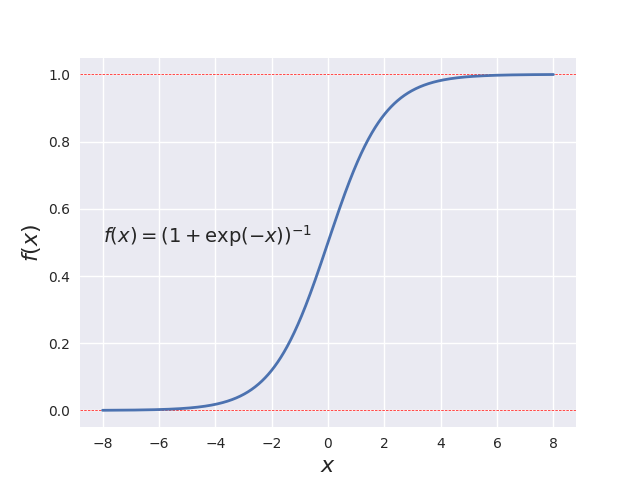
\includegraphics[width=8cm]{../plots/sigmoid.png} }}
	\subfloat[ReLU]{{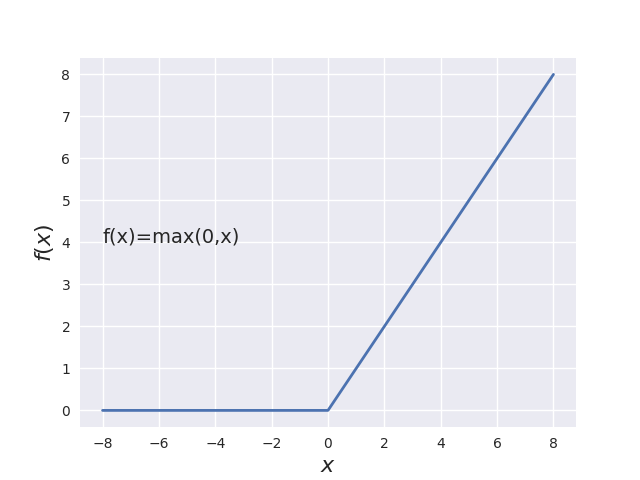
\includegraphics[width=8cm]{../plots/ReLU.png} }}\\
	
	\subfloat[Leaky ReLU]{{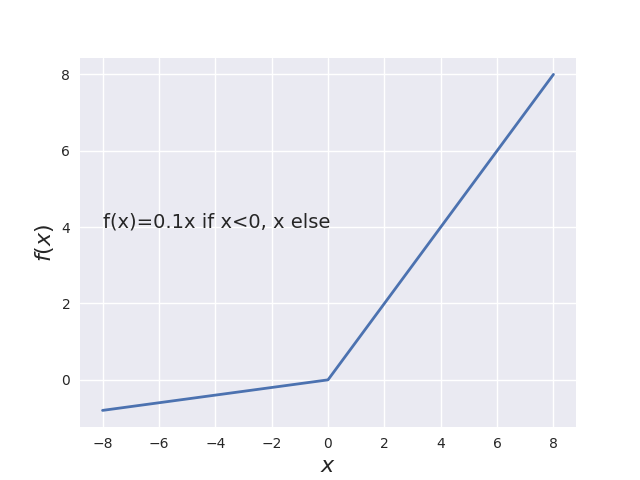
\includegraphics[width=8cm]{../plots/LeakyReLU.png} }}%
	\subfloat[ELU]{{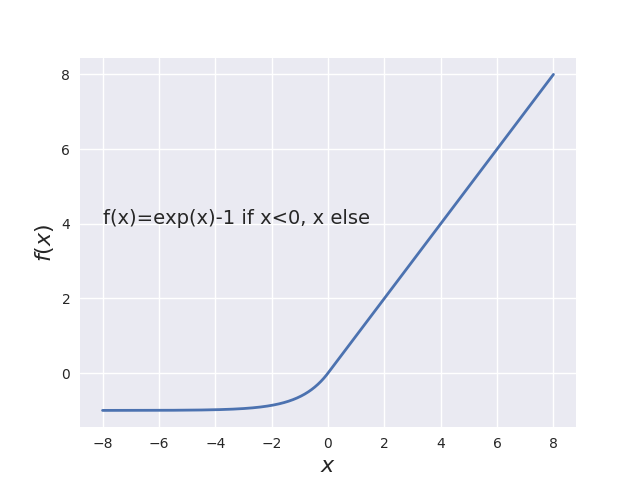
\includegraphics[width=8cm]{../plots/ELU.png} }}
	\caption{Some popular activation functions: the logistic activation function (a), ReLU function (b), Leaky ReLU function (c) and the ELU function (d). }%
	\label{fig:activation_functions}%
\end{figure}